\chapter{Proposed Methods}

The purpose of this experiment is to examine the hypothesis that a time-variant masking ratio would effects the prediction accuracy in text-based person retrieval tasks. We approach this by exploring the relationship between the sensitivity-aware representation learning, as investigated by \cite{Bai2023RaSaRA} in their work "RaSa," which focuses on improving representation learning for image and text inputs by detecting replaced tokens from the combined text and image inputs. Their results demonstrated significant improvements in prediction performance. They used masked language modeling to combine the image and text features to match the information, but the masking ratio was fixed to 15\% during the whole process.

To delve deeper into the impact of masking ratios, \cite{wettig-etal-2023-mask} suggested that larger models benefit from adopting a higher masking rate rather than the  conventional 15\% of tokens. Additionally, \cite{yang2023learningbettermaskingbetter} proposed a time-variant masking ratio decay strategy along with POS-tagging weighted masking. Their findings indicated that the time-variant masking decay method significantly outperformed the time-invariant masking ratio in terms of F1 score on the SQuAD dataset during the pre-training of the BERT-large model.

Our experiment aims to build on these insights by evaluating the effects of different masking strategies on the performance of vision-language models, specifically in the context of text-based person retrieval. By systematically varying the masking ratio and employing time-variant masking techniques, we seek to determine the optimal approach for enhancing the alignment and interpretation of textual and visual data.

% this part might not required
In this experiment, we investigate the effect of the performance towards the time variant masking ratio on replaced token detection task. To evaluate the performance, we compute the feature similarity score for all image-text pairs. Then, we take the top-$k$ candidates and calculate their ITM score $s_{itm}$ for ranking. 

\section{Dataset}

\begin{figure}[htbp]
  \begin{center}
      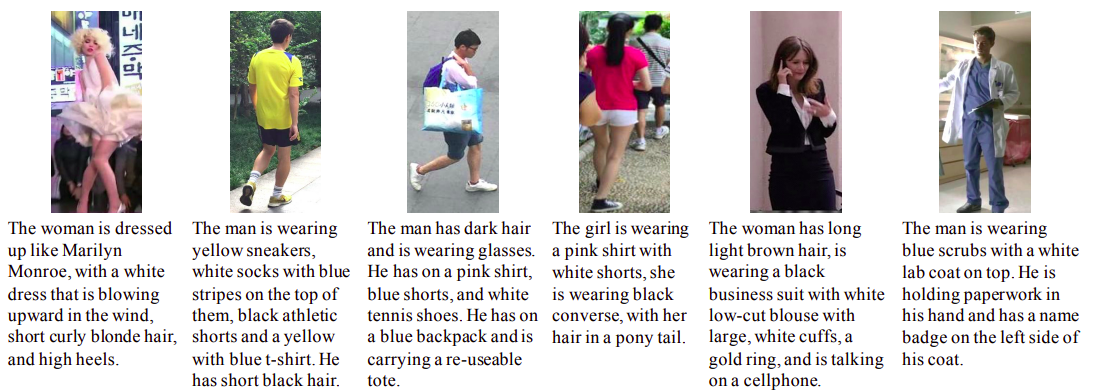
\includegraphics[width=\linewidth]{img/cuhk_pedes.png}
      \caption{Example sentence with corresponding images.}
      \label{fig:cuhk_pedes}
  \end{center}
\end{figure}


The dataset we are using is CUHK-PEDES (\cite{li2017personsearchnaturallanguage}). This is a large-scale dataset created to facilitate person search using natural language descriptions. It addresses the need for a dataset where persons are described in detail using natural language, enabling practical applications such as video surveillance. Key features of the dataset are shown as follows:
\begin{itemize}
  \item large-scale: the dataset contains 40,206 images of 13,003 persons; 
  \item annotations: each images is described with two sentences by independent annotators for a total of 80,412 sentence descriptions;
  \item source diversity: images are sourced from a variety of existing person re-identification datasets, including CUHK03 (\cite{li2014deepreid}), Market-1501 (\cite{7410490}), SSM (\cite{ssm}), VIPeR (\cite{viper}), and CUHK01 (\cite{li2012human}).
\end{itemize}

The datasets contain image and corresponding natural language description as shown in Fig\ref{fig:cuhk_pedes}. The image source for CUHK-PEDES are from CUHK03, Market-1501, SSM, VIPER, and CUHK01. The annotations for each image are done by Amazon Mechanical Turk (\acrshort{amt}) through crowd sourcing, where employees describe each image with two sentence. Each sentence includes rich descriptions about a person's appearance, action poses, and interactions.

\section{Methods}
In this section, we introduce the experimental methods designed to evaluate the performance of \acrshort{vlm}. Recent state-of-the-art VLMs, such as the one described by \cite{Bai2023RaSaRA} in their work `RaSa', utilize an attention mechanism to extract and align features from both images and text using cross-modality encoders. Achieving optimal results necessitates not only robust feature extraction but also the development of sophisticated textual representations to enhance the interpretation of visual data. Therefore, our objective is to train the visual-language model from RaSa by employing diverse strategies for textual information representation. Specifically, we will investigate two distinct methods to determine their impact on model performance.

% explain about the parameters based on the model image and loss function

\subsection{Masking Ratio for Masked Language Modeling} 
A Masked Language Model (MLM) is a type of neural network model used primarily for natural language processing tasks, including (\cite{devlin2018bert} and \cite{Bai2023RaSaRA}). MLMs are trained on text data where some of the words in the input sentences are replaced with a special token (often "[MASK]"), and the model's objective is to predict the original words that were masked. This training method helps the model learns to capture the semantics and syntax of the language, making it effective for various NLP tasks such as text classification, sentiment analysis, and machine translation.

During training, a portion of the input tokens are randomly masked, and the model learns to predict these masked tokens based on the surrounding context. For example, in the sentence "The cat sat on the [MASK]," the model should predict "mat" if it has learned the context correctly. For each image and text pair ($I,T^S$), MLM loss will be formulated as:
\[
  L_{mlm} = \mathbb{E}_{p \left( I,T^{msk}\right) }\mathrm{H}\left(y^{mlm}, \phi^{mlm}\left(I,T^{msk}\right)\right)
\]

Given a masked text \( T_{msk} \), where each token in the input text \( T_s \) is randomly masked with a probability \( p_m \), \( y_{mlm} \) represents a one-hot vector indicating the ground truth of the masked token. The function \( \phi_{mlm}(I, T_{msk}) \) denotes the predicted probability for the masked token, based on the context provided by the masked text \( T_{msk} \) and the paired image \( I \).

% explanation about what we do with masking ratio
In natural language pre-training, masked language modeling is utilized to understand the context of an input sentence. This same task is applied to recent vision-language models, where the masked token is predicted using both the image and the remaining text information. Although this method can yield good performance, the typical ratio for masking words in a sentence is fixed at 15\%. In our study, we aim to identify the optimal masking ratio by experimenting with time-invariant masking ratios ranging from 15\% to 40\%. Additionally, we will explore time-variant masking strategies based on previous findings to further enhance model performance.

Furthermore, we will evaluate the results by visual grounding with Grad-CAM (\cite{gradcam}) for Image text matching. This method is originally proposed for visual explanation in convolutional neural network (CNN). Grad-CAM utilizes gradients flowing into the convolutional layer to produce a localization map. The resulting gradient information is then used to weight the feature maps, which produces a heatmap that shows areas of the image that are most relevant to the prediction. The benefits of Grad-CAM is that the visualization is done by the gradient information, which does not require architectural changes or re-training of the network.

In this work, we will take the cross-attention maps in the 3rd layer of the multi-modal encoder (which is a layer specialized in grounding). The image is randomly taken from the test dataset, and input text will be defined with simple information.

\subsection{Fixed Masking Ratio}
We will train the model with constant masking ratio with range of 15\% to 40\% by 5\% steps with the dataset of CUHK-PEDES. Then, from the results, we will take the highest mean Average Precision (mAP) from the constant masking ratio and use that value with the minimum masking ratio. The minimum ratio will be 2\% since 0\% masking ratio will not train at all. 
{\color{red} may need refinement}
For all training tasks, the number of epochs is set to 30, and batch size is 13. The optimization methods used is adamW, the learning rate is set to $1.0e^4$ at first, and then decreases to $1.0e^5$ following a cosine curve pattern. Table 3.1 shows the results for masking with a fixed ratio, and table x shows the time variant masking ratio results.


\begin{table}[htbp]
\centering
  \caption{Result for masking fixed masking ratio}
  \begin{tabular}{rcccc}
    masking ratio & r1 & r5 & r10 & mAP\\ \hline
    15\% & 76.51 & \te-xtbf{90.20} & \textbf{94.25} & 69.38 \\
    20\% & 76.64 & 89.90 & 93.70 & 70.27 \\
    25\% & 76.23 & 89.86 & 93.79 & 70.22 \\
    30\% & \textbf{76.72} & 89.77 & 93.60 & \textbf{70.30} \\
    35\% & 76.61 & 89.77 & 93.47 & 70.26 \\
    40\% & 76.56 & 89.88 & 93.47 & 70.26
  \end{tabular}
\end{table}

\subsection{Time Variant Masking Ratio}
Time variant strategy will have the cosine curve and linear curve to see the result. The time variant will have four different methods, linear increase, linear decrease, cosine increase, and cosine decrease. The equations are shown as follows:
\begin{eqnarray}
M_{linear increase}\left( t \right) &=& P*t/T \\
M_{linear decrease}\left( t \right) &=& P*\left(1-t/T\right) \\
M_{cosine increase}\left(t\right) &=& P*\left(1-cos\left(\pi*t/T\right)\right) + 0.02 \\
M_{cosine decrease}\left(t\right) &=& P*\left(1+cos\left(\pi*t/T\right)\right) + 0.02 
\end{eqnarray}

\begin{figure}[htbp]
  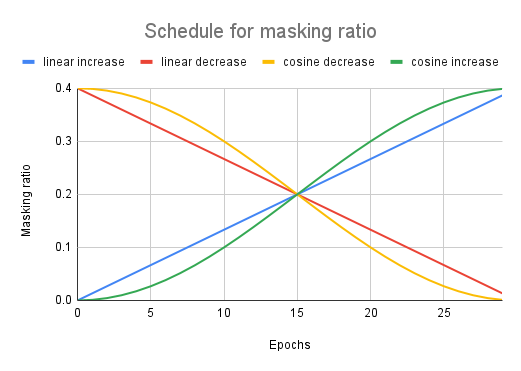
\includegraphics[width=\linewidth]{img/Schedule_masking_ratio.png}
  \caption{Masking Ratio Schedule for each methods}
  \label{img:masking_ratio_scheduler}
\end{figure}

\begin{table}[htbp]
  \centering
  \caption{Result for time variant masking ratio}
  \begin{tabular}{rcccc}
    \centering
    masking ratio & r1 & r5 & r10 & mAP\\ \hline
    linear increase & 76.62 & 89.88 & 93.62 & 70.36 \\
    linear decrease & 76.70 & 89.85 & 93.58 & 70.21 \\
    cosine increase & 76.54 & 90.04 & 94.02 & 70.15 \\
    cosine decrease & 76.21 & 90.09 & 93.65 & 70.21 \\
  \end{tabular}
\end{table}

{\color{red} fixed until here}
\section{Masking Ratio for Replaced Token Detection}
RaSa utilizes a loss function called replaced token detection to create a task called sensitivity aware learning.
Sensitivity aware aims to make the model sensitive to specific transformations in the data, particularly textual changes. While many models aim to learn invariant representations that are robust to various data augmentations, RaSa takes it further by encouraging the model to detect and respond to sensitive transformations, such as word replacements in text. This is done using a Momentum-based Replaced Token Detection (M-RTD) task, where the model learns to detect whether a token in the text has been replaced. This sensitivity to changes enhances the robustness and discrimination power of the representations learned by the model.
{\color{red}further explanation about sensitivity aware}


\begin{table}[htbp]
  \centering
  \caption{Result for fixed masking ratio on m-RTD}
  \begin{tabular}{rcccc}
    masking ratio & r1 & r5 & r10 & mAP \\ \hline
    15\% & 75.42 & 90.20 & 93.83 & 68.56 \\
    20\% & 75.58 & 90.35 & 93.91 & 68.73 \\
    25\% & 75.63 & 90.09 & 93.83 & 68.76 \\
    30\% & 75.57 & 93.92 & 93.92 & 68.81 \\
    35\% & 75.03 & 90.14 & 93.89 & 68.57 \\
    40\% & 75.80 & 90.27 & 93.97 & 68.73
  \end{tabular}
\end{table}

Predicting more means the model learns from more training signals, so higher prediction rates boost the model performance. From another perspective, each prediction at each masked token leads to a loss gradient, which is averaged to optimize the weights of the model. Averaging across more predictions has a similar effect to increasing the batch size, which is proven to be beneficial for pre-training (Liu et al., 2019). 

\section{Attention Visualization}
To be able to see where the model is paying attention to, we use the attention matrix in cross attention module. 

Ramprasaath R. Selvaraju et al. present a method for providing visual explanations for the decisions made by Convolutional Neural Networks (CNNs). This method, called Gradient-weighted Class Activation Mapping (Grad-CAM), generates a coarse localization map that highlights important regions in an image crucial for predicting a specific concept.

Grad-CAM utilizes gradients flowing into the final convolutional layer to produce a localization map. It is applicable to various CNN architectures, including those with fully-connected layers (like VGG), and models for structured outputs. When combined with pixel-space gradient visualizations, Grad-CAM creates Guided Grad-CAM, which offers high-resolution, class-discriminative visualizations.

Following steps enables to obtain the class-discriminative localization map $L^c_{Grad-CAM} = \in\Re^{u \times v}$ of class $c$ from the image width $u$ and height $v$. 

First, we would define the neuron importance weights $\alpha^c_k$. calculate the gradient of the score for class c, $y_c$(before softmax), with respect to the feature map activations $A_k$ of a convolutional layer, i.e., $\frac{\delta y^c}{\delta A^k}$. 
 
\begin{displaymath}
    L^c_{Grad-CAM} = ReLU(\sum_k\alpha^c_kA^k)
\end{displaymath}

One significant advantage of this method is its class-discriminative nature. Grad-CAM can highlight specific regions relevant to a particular class, making it useful for understanding model predictions. Another advantage is the high resolution of the visualizations. By combining Grad-CAM with existing fine-grained visualization techniques like Guided Backpropagation, the authors create Guided Grad-CAM, which provides detailed and class-discriminative visual explanations.

Below are the results achieved from the MLM with different masking ratio.

\begin{figure}[htbp]
  
\includegraphics[width=\linewidth]{img/placeholder.png}
  \caption{placeholder for visual grounding on MLM}
\end{figure}

Below are the results achieved from the m-RTD with different masking ratio.
\begin{figure}[htbp]
  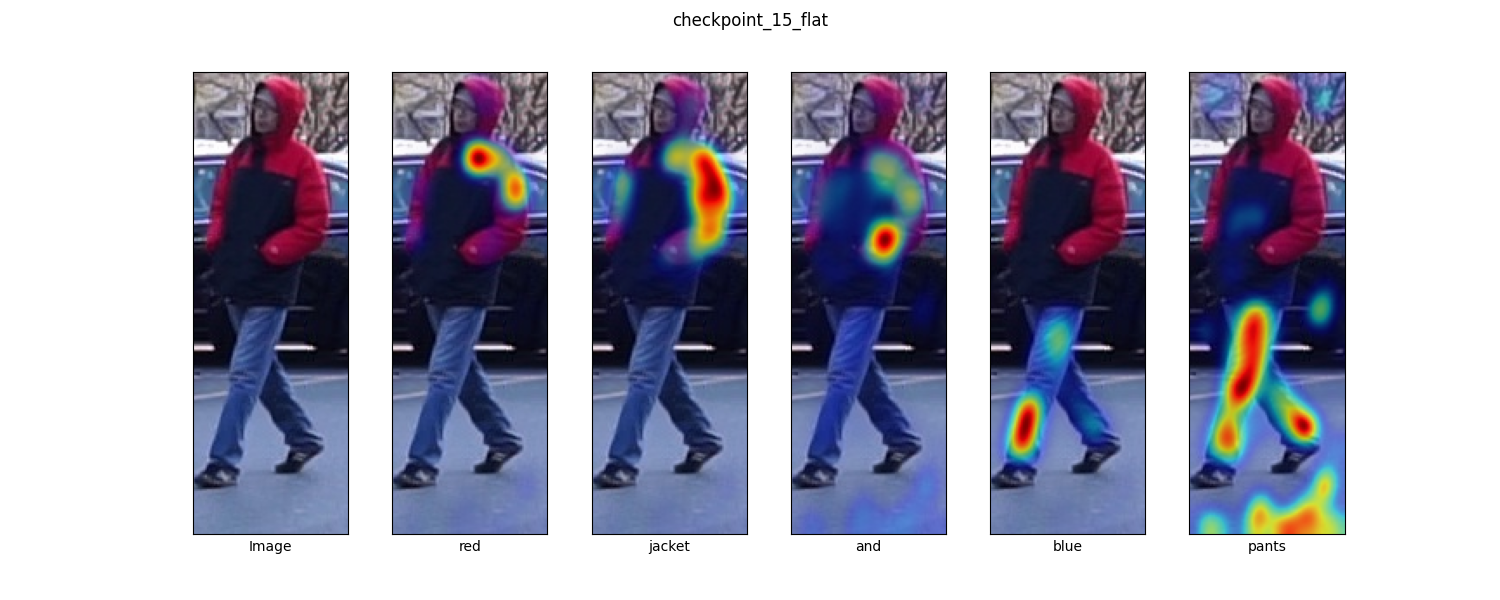
\includegraphics[width=\linewidth]{img/mrtd_masking_ratio/mrtd-checkpoint_15_flat.png}
  \caption{Visual grounding for masking rate of 15}
\end{figure}

\begin{figure}[htbp]
  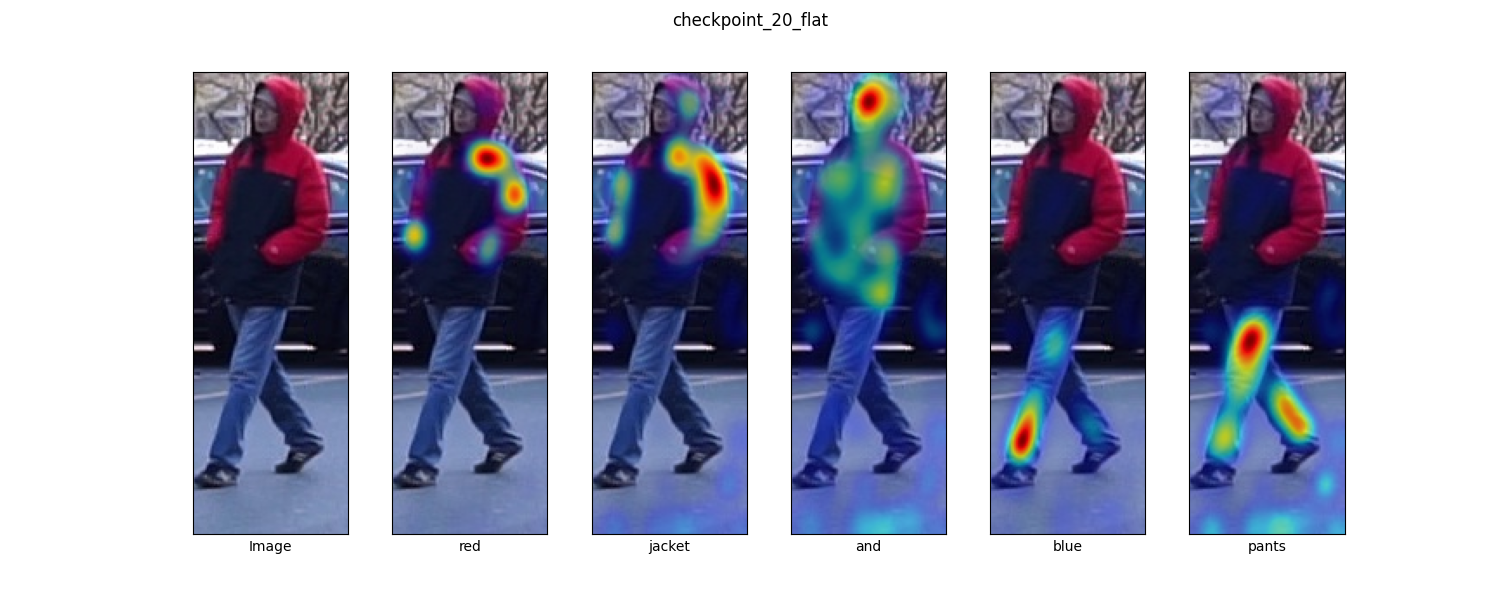
\includegraphics[width=\linewidth]{img/mrtd_masking_ratio/mrtd-checkpoint_20_flat.png}
  \caption{Visual grounding for masking rate of 20}
\end{figure}

\begin{figure}[htbp]
  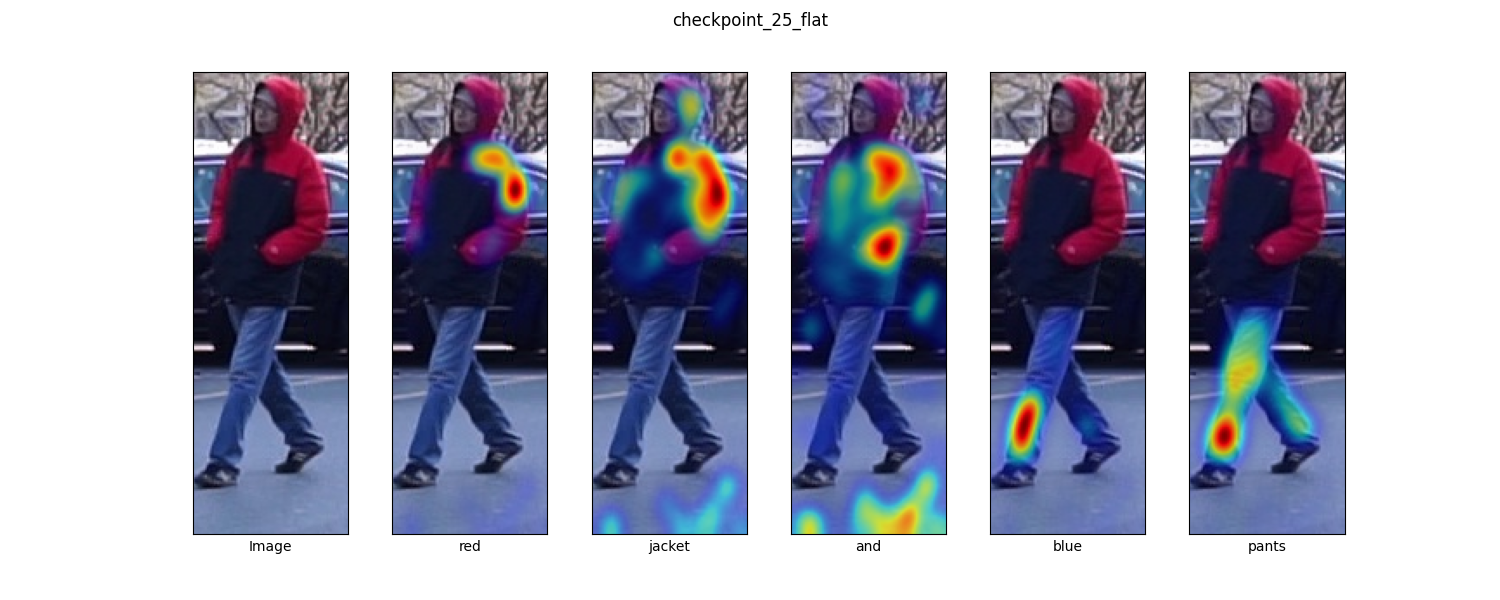
\includegraphics[width=\linewidth]{img/mrtd_masking_ratio/mrtd-checkpoint_25_flat.png}
  \caption{Visual grounding for masking rate of 25}  
\end{figure}

\begin{figure}[htbp]
  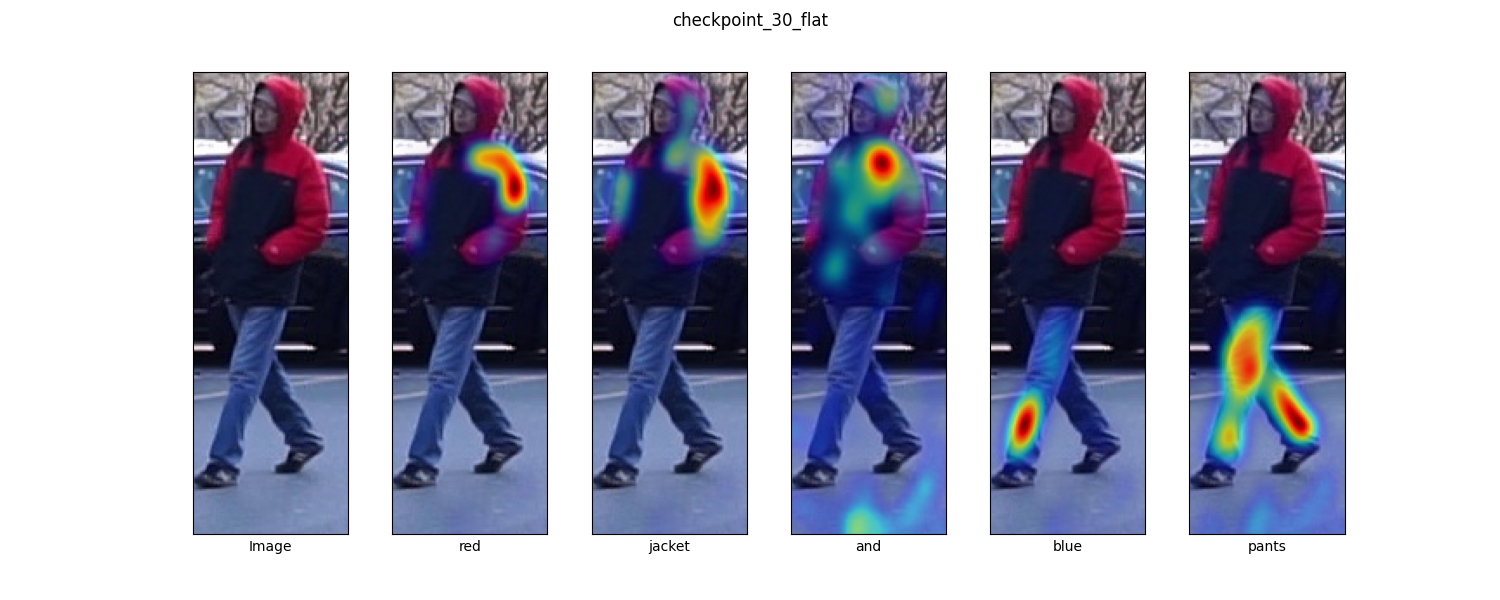
\includegraphics[width=\linewidth]{img/mrtd_masking_ratio/mrtd-checkpoint_30_flat.png}
  \caption{Visual grounding for masking rate of 30}
\end{figure}

\begin{figure}[htbp]
  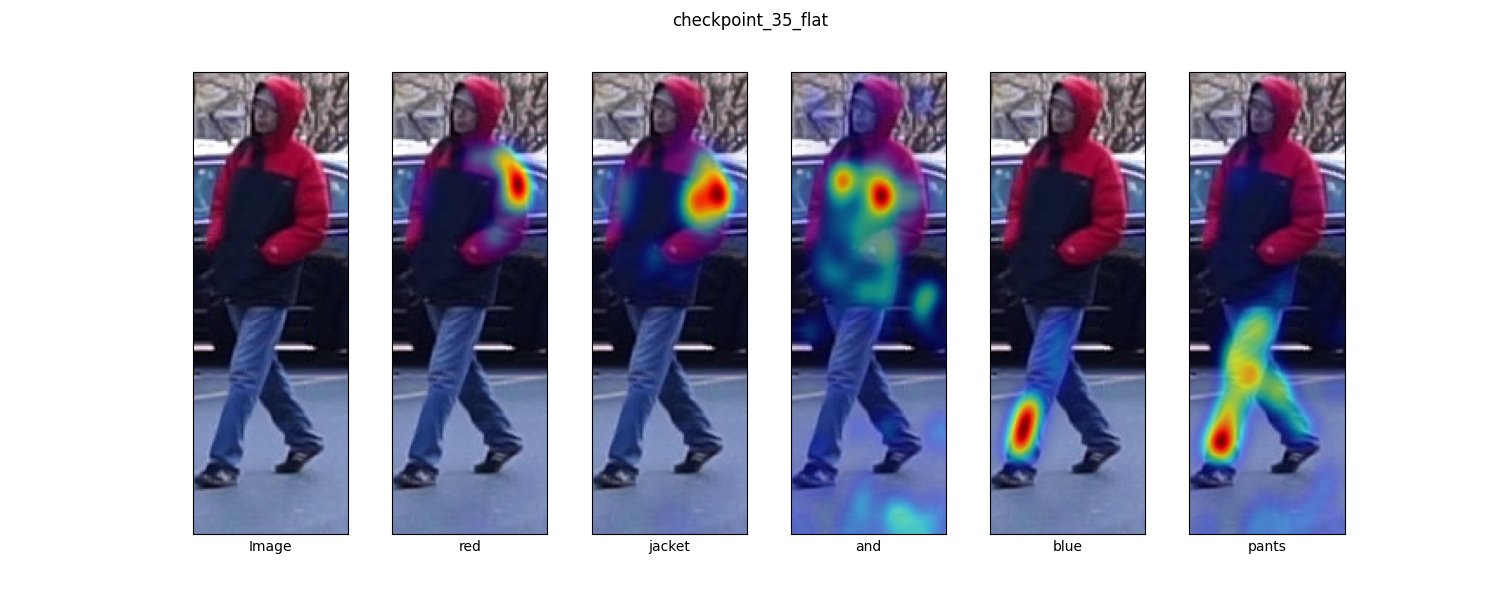
\includegraphics[width=\linewidth]{img/mrtd_masking_ratio/mrtd-checkpoint_35_flat.png}
  \caption{Visual grounding for masking rate of 35}
\end{figure}

\begin{figure}[htbp]
  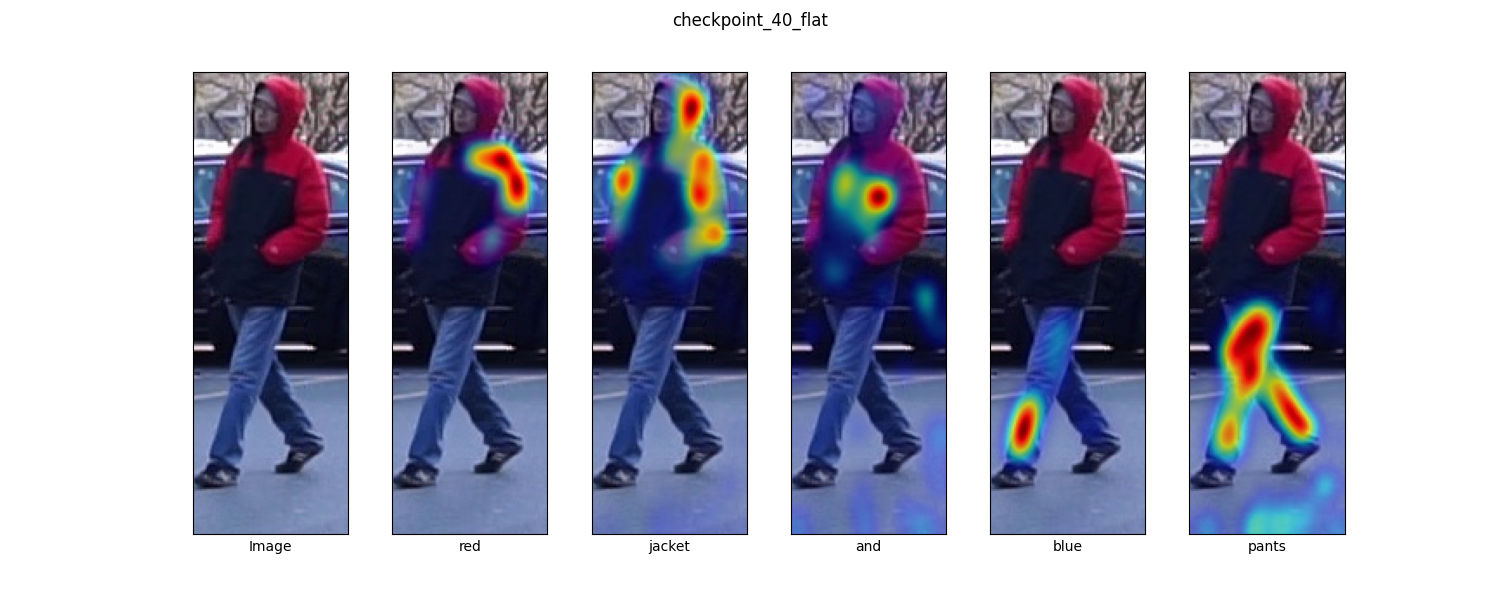
\includegraphics[width=\linewidth]{img/mrtd_masking_ratio/mrtd-checkpoint_40_flat.png}
  \caption{Visual grounding for masking rate of 40}
\end{figure}